\documentclass{article}
\usepackage[margin=1in]{geometry}
\usepackage{amsmath,amsthm,amssymb}
\usepackage{bbm,enumerate,mathtools}
\usepackage{tikz,pgfplots}
\usepackage{chessboard}
\usepackage[hidelinks]{hyperref}
\usepackage{multicol} % Problem 35
\usepackage{xstring} % Difficulty command
\usetikzlibrary{shapes.geometric}

\newenvironment{question}{\begin{trivlist}\item[\textbf{Question.}]}{\end{trivlist}}
\newenvironment{note}{\begin{trivlist}\item[\textbf{Note.}]}{\end{trivlist}}
\newenvironment{references}{\begin{trivlist}\item[\textbf{References.}]}{\end{trivlist}}
\newenvironment{related}{\begin{trivlist}\item[\textbf{Related.}]\end{trivlist}\begin{enumerate}}{\end{enumerate}}

\newcommand\score[1]{
\pgfmathsetmacro\pgfxa{#1+1}
\tikzstyle{scorestars}=[
  star,
  star points=5,
  star point ratio=2.25,
  draw,
  inner sep=3pt,
  anchor=outer point 5
]
  \begin{tikzpicture}[baseline]
    \draw[opacity=0] (0,-0.5) rectangle (0,0.2); % Workaround for whitespace at the bottom.
    \foreach \i in {1,...,4} {
      \pgfmathparse{(\i<=#1?"yellow":"gray")}
      \edef\starcolor{\pgfmathresult}
      \draw (\i*4.5ex,0) node[name=star\i,scorestars,fill=\starcolor]  {};
    }
  \end{tikzpicture}
}

\newcommand{\difficulty}[1]{%
  \IfEqCase{#1}{%
      {1}{
        
\begin{tikzpicture}[scale=0.7, baseline=0.9mm]%
          \definecolor{slopegreen}{rgb}{0.0, 0.5, 0.0}%
          \fill[slopegreen] (0.5,0.5) circle (0.5);%
        \end{tikzpicture}%
      }%
      {2}{
        
\begin{tikzpicture}[scale=0.7, baseline=0.9mm]%
          \definecolor{slopeblue}{rgb}{0.0, 0.44, 1.00}
          \fill[slopeblue] (0,0) rectangle (1,1);%
        \end{tikzpicture}%
      }%
      {3}{
\begin{tikzpicture}[scale=0.7, baseline=0.9mm]\fill (0,0.5)--(0.5, 0)--(1,0.5)--(0.5,1)--cycle; \end{tikzpicture}}%
      {4}{
\begin{tikzpicture}[scale=0.7, baseline=0.9mm]\fill (0.25,0)--(0,0.5)--(0.25,1)--(0.5,0.5)--cycle; \fill (0.75,0)--(0.5,0.5)--(0.75,1)--(1,0.5)--cycle;\end{tikzpicture}}%
      % you can add more cases here as desired
  }[\PackageError{difficulty}{Undefined difficulty level: #1}{}]%
}%
\newcommand{\rating}[2]{\difficulty{#1}\\\score{#2}\\}


\begin{document}
\rating{2}{1}
Say that two sequences with distinct elements are in the same equivalence
class if their first differences have the same signs.
(e.g. $(1, 3, 2, 3)$ and $(7,8,-1,0)$ are equivalent because their first
differences are both $(+, -, +)$.)
\begin{figure}[!h]
  \centering
  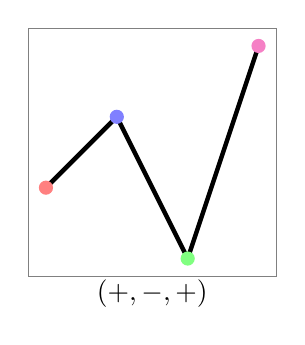
\begin{tikzpicture}[scale = 0.9]
    \draw[gray] (-0.25, -1.25) rectangle (3.25, 2.25);
    \draw[ultra thick](0,0)--(1,1)--(2,-1)--(3,2);
    \fill[red!50] (0,0) circle (0.1cm);
    \fill[blue!50] (1,1) circle (0.1cm);
    \fill[green!50] (2,-1) circle (0.1cm);
    \fill[magenta!50] (3,2) circle (0.1cm);
    \node at (1.5, -1.5) {$(+, -, +)$};
  \end{tikzpicture}\hspace{0.5cm}
  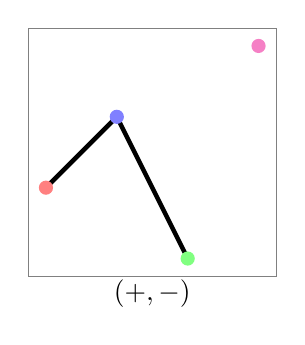
\begin{tikzpicture}[scale = 0.9]
    \draw[gray] (-0.25, -1.25) rectangle (3.25, 2.25);
    \draw[ultra thick](0,0)--(1,1)--(2,-1);
    \fill[red!50] (0,0) circle (0.1cm);
    \fill[blue!50] (1,1) circle (0.1cm);
    \fill[green!50] (2,-1) circle (0.1cm);
    \fill[magenta!50] (3,2) circle (0.1cm);
    \node at (1.5, -1.5) {$(+, -)$};
  \end{tikzpicture}\hspace{0.5cm}
  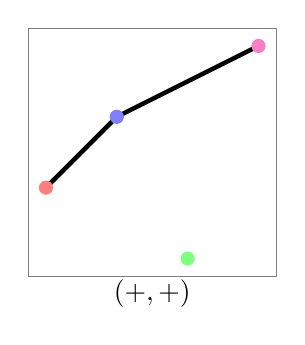
\begin{tikzpicture}[scale = 0.9]
    \draw[gray] (-0.25, -1.25) rectangle (3.25, 2.25);
    \draw[ultra thick](0,0)--(1,1)--(3,2);
    \fill[red!50] (0,0) circle (0.1cm);
    \fill[blue!50] (1,1) circle (0.1cm);
    \fill[green!50] (2,-1) circle (0.1cm);
    \fill[magenta!50] (3,2) circle (0.1cm);
    \node at (1.5, -1.5) {$(+, +)$};
  \end{tikzpicture}\\\vspace{0.5cm}
  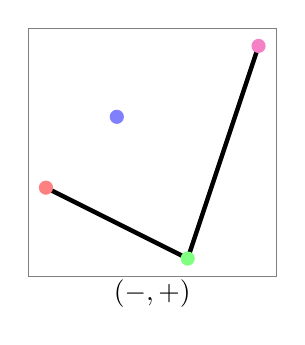
\begin{tikzpicture}[scale = 0.9]
    \draw[gray] (-0.25, -1.25) rectangle (3.25, 2.25);
    \draw[ultra thick](0,0)--(2,-1)--(3,2);
    \fill[red!50] (0,0) circle (0.1cm);
    \fill[blue!50] (1,1) circle (0.1cm);
    \fill[green!50] (2,-1) circle (0.1cm);
    \fill[magenta!50] (3,2) circle (0.1cm);
    \node at (1.5, -1.5) {$(-, +)$};
  \end{tikzpicture}\hspace{0.5cm}
  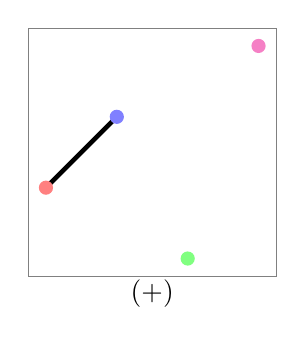
\begin{tikzpicture}[scale = 0.9]
    \draw[gray] (-0.25, -1.25) rectangle (3.25, 2.25);
    \draw[ultra thick](0,0)--(1,1);
    \fill[red!50] (0,0) circle (0.1cm);
    \fill[blue!50] (1,1) circle (0.1cm);
    \fill[green!50] (2,-1) circle (0.1cm);
    \fill[magenta!50] (3,2) circle (0.1cm);
    \node at (1.5, -1.5) {$(+)$};
  \end{tikzpicture}\hspace{0.5cm}
  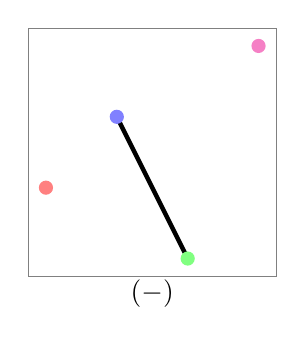
\begin{tikzpicture}[scale = 0.9]
    \draw[gray] (-0.25, -1.25) rectangle (3.25, 2.25);
    \draw[ultra thick](1,1)--(2,-1);
    \fill[red!50] (0,0) circle (0.1cm);
    \fill[blue!50] (1,1) circle (0.1cm);
    \fill[green!50] (2,-1) circle (0.1cm);
    \fill[magenta!50] (3,2) circle (0.1cm);
    \node at (1.5, -1.5) {$(-)$};
  \end{tikzpicture}
  \caption{
    $(0, 1, -1, 2)$ has subsequences in the following six equivalence classes:
    $(+, -, +)$, $(+, +)$, $(+, -)$, $(-, +)$, $(+)$, $(-)$. No length $4$
    sequence has its subsequences in more equivalence classes, so $a(4) = 6$.
  }
\end{figure}

\begin{question}
  What is the general formula for $a(n)$?
\end{question}
\begin{related}
  \item What if the sequences do not necessarily consist of distinct elements?
  \item What if two sequences are considered to be equivalent if they are in the
    same ``sort order''; that is, if both sequences have their biggest element
    in the same position, their second biggest in the same position, and so on.
  \item What if $(+, +) \sim (+)$?
  \item Is the number of equivalence classes for the subsequences determined by
   the number of local minima and maxima?
\end{related}

\begin{note}
  A quick attempt finds that $a(2) = 1$, $a(3) = 3$, $a(4)=6$, and $a(5)=11$.
  (Fibonacci minus 2?)\\
  For related question 3, conjecture the answer is $a'(n) = 2n - 3$ for $n \geq 2$.\\
  For related question 3 without distinct elements (as in related question 1),
  the inital terms are
  \begin{align*}
    a(2) &= 1 \text { via } (+)  \\
    a(3) &= 4 \text { via } (+, -), (+), (-), (=)  \\
    a(4) &= 8 \text { via } (+, -, +), (+, -), (+, =), (=, +), (-, _) (+), (-), (=)  \\
    a(5) &= 15; a(6) = 25; a(7) = 40\\
    a(8) &= 62; a(9) = 94; a(10) = 141; a(11) = 210; a(12) = 311 \text{ (conjectured*)}
  \end{align*}
  * Assumes sequence is $(1,2,1,2,1,2,\hdots)$.
\end{note}

\end{document}
